%%%%%%%%%%%%%%%%%%%%%%%%%%%%%%%%%%%%%%%%%%%%%%%%%%%%%%%%%%%%%%
% ECE 445 SENIOR DESIGN TEMPLATE
%%%%%%%%%%%%%%%%%%%%%%%%%%%%%%%%%%%%%%%%%%%%%%%%%%%%%%%%%%%%%
\documentclass[letterpaper,10pt]{article}

%%%%%%%%%%%%%%%%%%%%%%%%%%%%%%%%%%%%%%%%%%%%%%%%%%%%%%%%%%%%%
% The preamble starts here.
% You can add other packages that you want to use by using
% \usepackage command in the preamble.
% However, DO NOT change the settings that are already placed
% below unless you really know what you are doing.
%%%%%%%%%%%%%%%%%%%%%%%%%%%%%%%%%%%%%%%%%%%%%%%%%%%%%%%%%%%%%

% some commonly used packages
\usepackage{siunitx}
\usepackage{tikz}
\usepackage{listings}
\usepackage{graphicx}
\usepackage{color,soul}
\usepackage{amsmath}
\usepackage{amsthm}
\usepackage{amsfonts}
\usepackage{setspace}
\usepackage{longtable}
\usepackage{url}
\usepackage{pdfpages}
\usepackage{float}
\usepackage{rotating}
\usepackage{caption}
\usepackage{booktabs}  % professional-looking tables
\usepackage{multicol} %used for getting multicolumn without page-break
\usepackage{multirow}	% multi-row tables
\usepackage{array}		% define column format of a table
\usepackage[colorlinks=true,linkcolor=black,citecolor=black]{hyperref}
\usepackage[top=1.1in, bottom=1.1in, left=1.1in, right=1.1in]{geometry}% set the page margins to 1 inch

\lstset{frame=tb,
	language=C,
	aboveskip=3mm,
	belowskip=3mm,
	showstringspaces=false,
	columns=flexible,
	basicstyle={\small\ttfamily},
	numbers=none,
	numberstyle=\tiny\color{gray},
	keywordstyle=\color{blue},
	commentstyle=\color{dkgreen},
	stringstyle=\color{mauve},
	breaklines=true,
	breakatwhitespace=true,
	tabsize=3
}

\usepackage{color}
\definecolor{dkgreen}{rgb}{0,0.6,0}
\definecolor{gray}{rgb}{0.5,0.5,0.5}
\definecolor{mauve}{rgb}{0.58,0,0.82}

% use the fancyhdr package to maintain the format of the page numbers,
% which is useful when the text color is changed
\usepackage{fancyhdr}
\fancyhf{}
\renewcommand{\headrulewidth}{1pt}
\renewcommand{\footrulewidth}{0pt}
\fancyfoot[C]{\textcolor{black}{\thepage}}
\fancyhead[L]{
\includegraphics[width=2cm]{University-of-Illinois-logo.jpg}}
\fancyhead[R]{\small{Infantry I.F.F. Individual Progress Report - Meyers}}

% paralist provides extended list environments
\usepackage{paralist}
\setlength{\plitemsep}{0pt}

% define the color for section and subsection titles
\usepackage{xcolor}
\definecolor{titlecolor}{RGB}{31,73,125}
\definecolor{subtitlecolor}{RGB}{79,129,189}

% change the style of the section and subsection titles
\usepackage{titlesec}
\titleformat{\section}{\color{titlecolor}\Large\bf}{\color{titlecolor}\thesection}{0.8em}{}
\titleformat{\subsection}{\color{subtitlecolor}\large\bf}{\color{subtitlecolor}\thesubsection}{1em}{}
\titleformat{\subsubsection}{\color{subtitlecolor}\normalsize\bf}{\color{subtitlecolor}\thesubsubsection}{1.2em}{}
\titlespacing{\section}{0pt}{0em}{0em}
\titlespacing{\subsection}{6pt}{0em}{0em}
\titlespacing{\subsubsection}{12pt}{0em}{0em}



% change the style of the table of contents
\usepackage{titletoc}
\titlecontents{section}[1.5em]{}{\contentslabel{1.5em}}{\hspace*{-1.5em}}{\titlerule*[0.5pc]{.}\contentspage}
\titlecontents{subsection}[3em]{}{\contentslabel{2.1em}}{\hspace*{-2.1em}}{\titlerule*[0.5pc]{.}\contentspage}
\titlecontents{subsubsection}[5.1em]{}{\contentslabel{2.7em}}{\hspace*{-2.7em}}{\titlerule*[0.5pc]{.}\contentspage}

% command for centering texts in a fixed width table cell
\newcommand{\centpcol}{\leftskip\fill \rightskip\fill}

% command for setting the style of the appendix titles
\newcommand{\setappenstyle}{
	\titleformat{\section}{\color{titlecolor}\Large\bf}{\color{titlecolor}Appendix \Alph{section}}{0.8em}{}
	\titlecontents{section}[0em]{}{Appendix \thecontentslabel \hspace{1em}}{}{\titlerule*[0.5pc]{.}\contentspage}
}

\makeatletter
\newcommand{\skipitems}[1]{%
	\addtocounter{\@enumctr}{#1}%
}

% define the style of the title of the paper
\newcommand{\thetitle}[1]{\title{\begin{huge}{\bf #1}\end{huge} \color{subtitlecolor}\rule[25pt]{\textwidth}{1pt}}}

% define the style of the author
\newcommand{\theauthor}[3]{
	\author{\vspace{.4in}\\
	\textcolor{black}{By}\\
	#1
	\vspace{1in}\\
	\textcolor{black}{ECE 445 Individual Progress Report -} #2\\
	\textcolor{black}{TA:} #3
	\vspace{1in}}
}

% define the style of figure's caption
\newcommand{\figcap}[1]{
	\captionsetup{format=plain,font={small,color=subtitlecolor,singlespacing},margin={0pt,0pt}}
	\caption{\textcolor{subtitlecolor}{#1}}
	\vspace{-5pt}
}

% define the style of table's caption
\newcommand{\tablecap}[1]{
	\captionsetup{format=plain,font={bf,normalsize,singlespacing,color=black},margin={0pt,0pt}}
	\caption{\textcolor{black}{#1}}
	\vspace{-5pt}
}


\newcommand{\buildtoc}{
	\clearpage
	\singlespacing
	\tableofcontents
	\onehalfspacing
}

% set indentations and the space between paragraghs
\setlength{\parindent}{0pt}
\setlength{\parskip}{8pt}

\setcounter{secnumdepth}{4}

\titleformat{\paragraph}
{\normalfont\small\bfseries\color{subtitlecolor}}{\theparagraph}{1em}{}
\titlespacing*{\paragraph}
{18pt}{3.25ex plus 1ex minus .2ex}{1.5ex plus .2ex}

%%%%%%%%%%%%%%%%%%%%%%%%%%%%%%%%%%%%%%%%%%%%%%%%%%%%%%%%%%%%%
% PREAMBLE ENDS HERE, DOCUMENT STARTS BELOW
%%%%%%%%%%%%%%%%%%%%%%%%%%%%%%%%%%%%%%%%%%%%%%%%%%%%%%%%%%%%%

\begin{document}

% don't change these
\pagestyle{empty}
\doublespacing

% put the title of your project here. DO NOT include the brackets.
\thetitle{{I.F.F. (Identification Friend or Foe) System}}

% put your names here. seperate by \\. DO NOT include the brackets.
\theauthor{
	{Eric Meyers (emeyer7)}\\
}
{ % put the semester info here. DO NOT include the brackets.
	{Spring 2016}
}
{ % put your TA's name here. DO NOT include the brackets.
	{Braedon Salz}
}

% put the date and project number here. DO NOT include the brackets.
\date{
{March 28th, 2016}\\
Project No. 11
\clearpage
}

% don't change these
\maketitle
\pagestyle{fancy}
\begin{spacing}{1.15}


% build the table of contents. 
\color{black}
\buildtoc
\pagenumbering{gobble}
\clearpage
\setcounter{page}{1}
\pagenumbering{arabic}

%SECTION - Introduction
\section{Introduction}
\subsection{Overview}
An Infantry I.F.F. System is a difficult yet very interesting project to tackle and many approaches were considered during the brainstorming period. In the end, the team decided to devise a two-way communication system that any soldier may wear and mount to their weapon that queries a target. Upon receiving this query, the target must send back an encrypted message to the interrogator to verify that it is friendly. 

\subsection{Personal Involvement}
The team purposefully split this project into two sub-units called the "friendly interrogator unit" and the "friendly target unit" so that the work could be evenly divided amongst the two of us. Throughout the past 8 weeks, I have been primarily working on the friendly interrogator unit as well as software for the MSP430 microcontroller.


The following accomplishments have been made since the Design Review for this project:

\begin{itemize}
	\item Circuit Schematic \& PCB for Friendly Interrogator Unit
	\item Circuit Schematic \& PCB for MSP430 TSSOP-to-DIP Adapter
	\item Microcontroller, Voltage Regulator, Crystal Oscillator, R.F. Equipment Ordered
	\item MSP430 Software Researched and Written (Unit Tests Included)
\end{itemize}

These will be expanded upon in the design section below. 

%SECTION - Design
\section{Design}

%DESIGN - FRIENDLY INTERROGATOR UNIT
\subsection{Overview} \label{section-friendly-interrogator-design}
One may refer to the figure in the Design Review of this project labeled "Block Diagram of Friendly Interrogator Unit" to get a high-level understanding of how the friendly interrogator unit functions. 

%Subsection - Circuit Schematics
\subsection{Circuit Schematics} \label{section-circuit-schematics}

\subsubsection{Friendly Interrogator Unit}
The circuit schematic for the friendly interrogator unit is broken into 4 primary modules for schematic viewing: the AAT1217 DC-DC step-up converter, the crystal oscillator, the MCU/laser transmitter/LED indicator/power switches, and the R.F. receiver/decoder circuits. These are displayed below.
\begin{figure} [H]
	\centering
	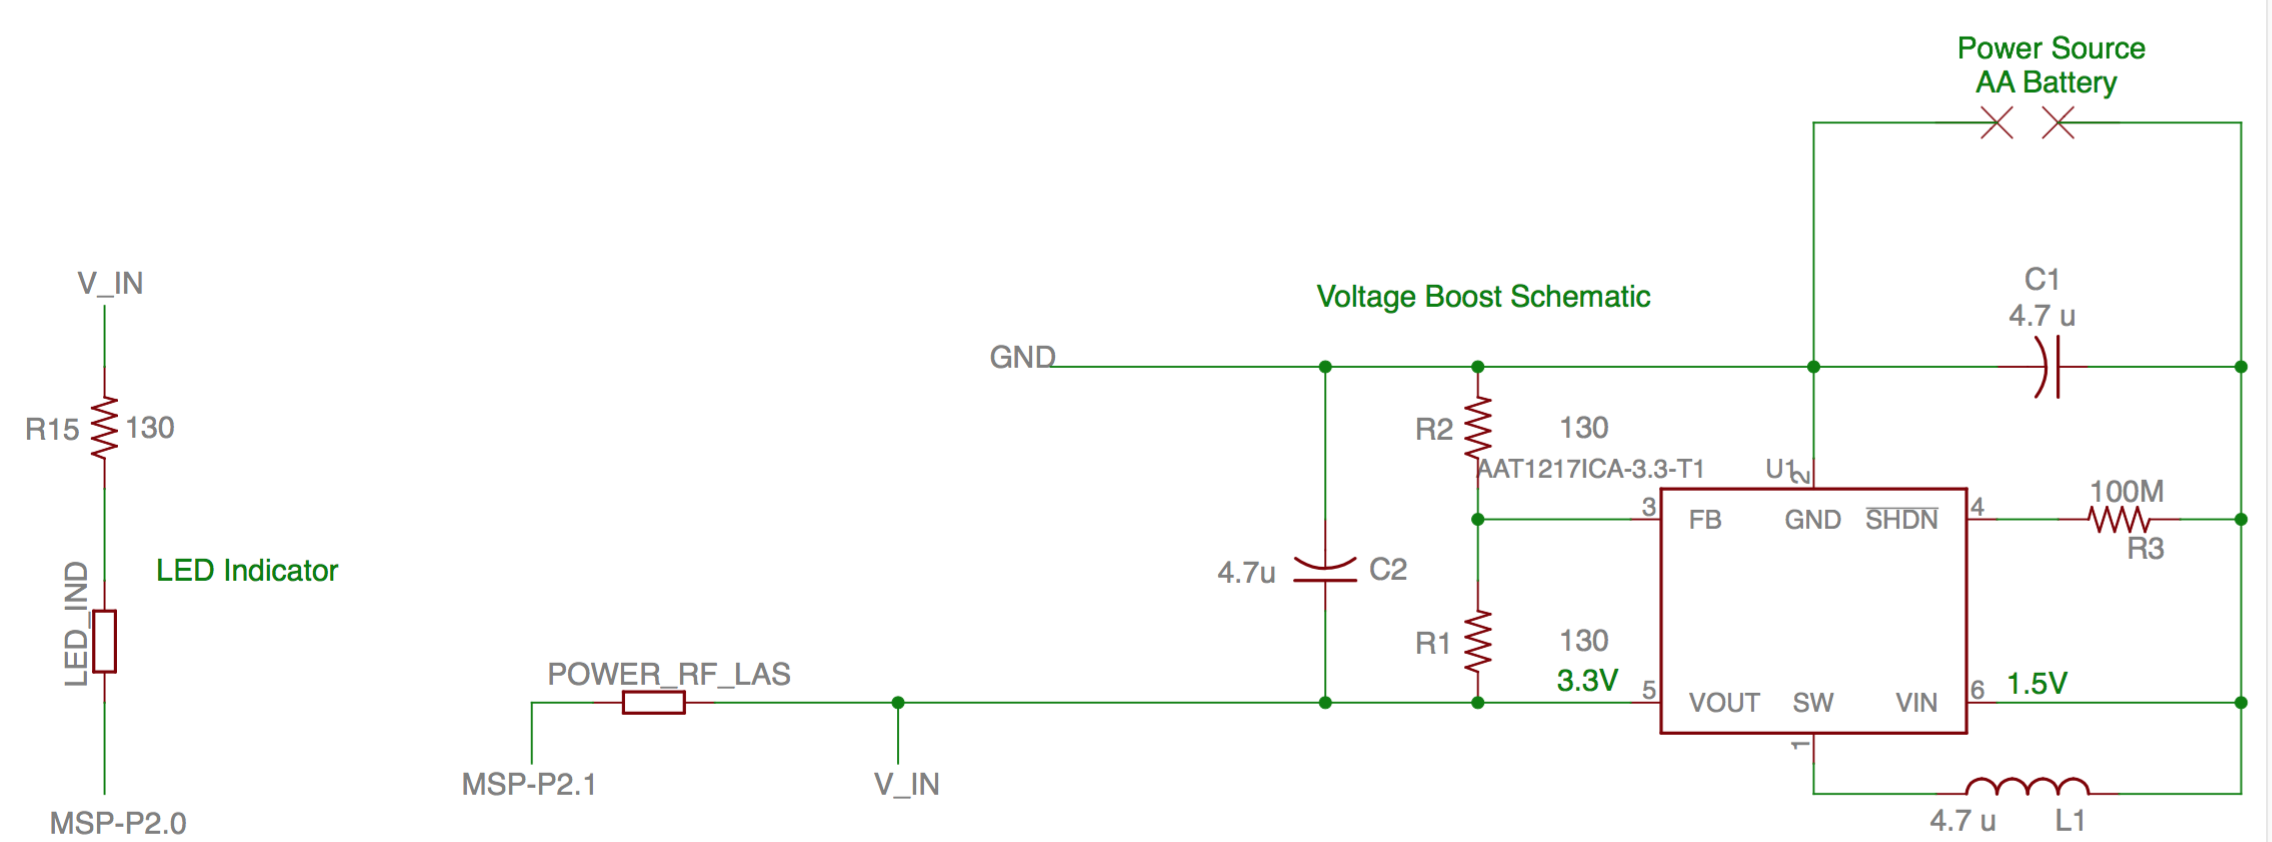
\includegraphics[scale=0.35]{converter-schematic.png}
	\caption{AAT1217 Circuit Schematic\label{fig:voltage-converter-schematic}}
\end{figure}

\begin{figure} [H]
	\centering
	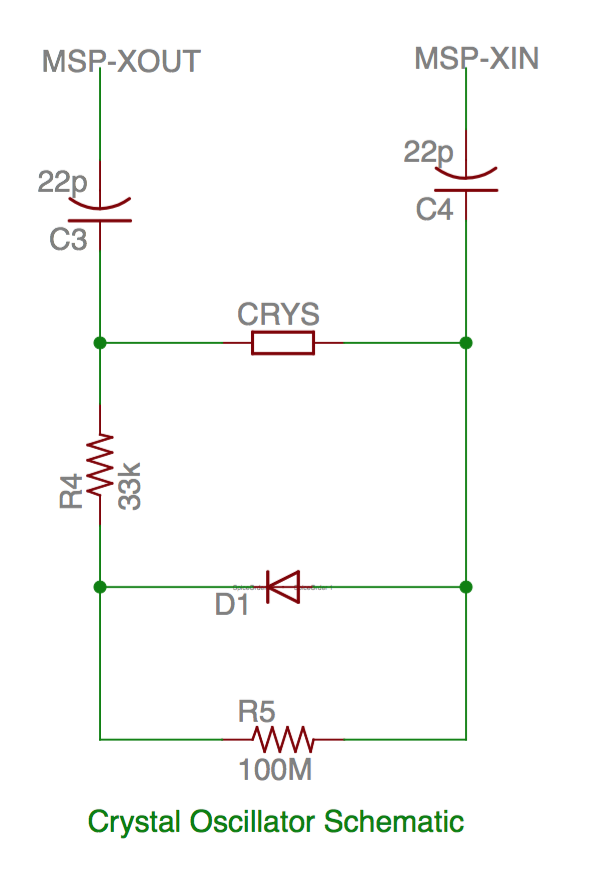
\includegraphics[scale=0.35]{oscillator-schematic.png}
	\caption{Crystal Oscillator Real Time Clock Circuit Schematic\label{fig:crystal-oscillator-schematic}}
\end{figure}

\begin{figure} [H]
	\centering
	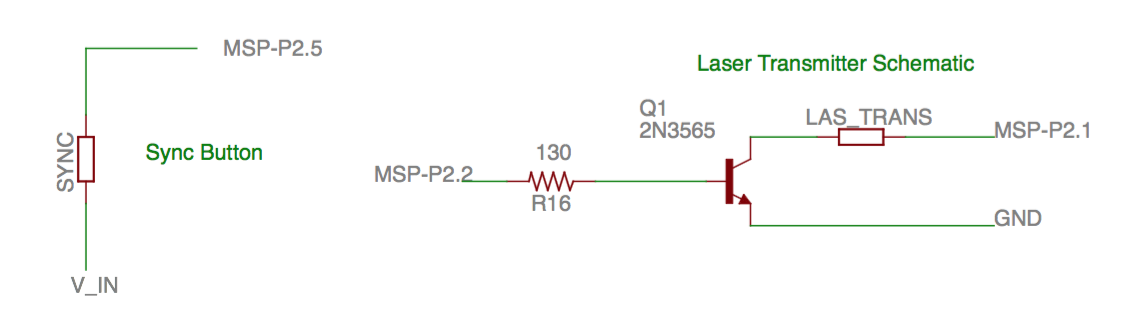
\includegraphics[scale=0.43]{transmitter-schematic.png}
	\caption{MCU and Laser Transmitter Circuit Schematic\label{fig:mcu-laser-schematic}}
\end{figure}

\begin{figure} [H]
	\centering
	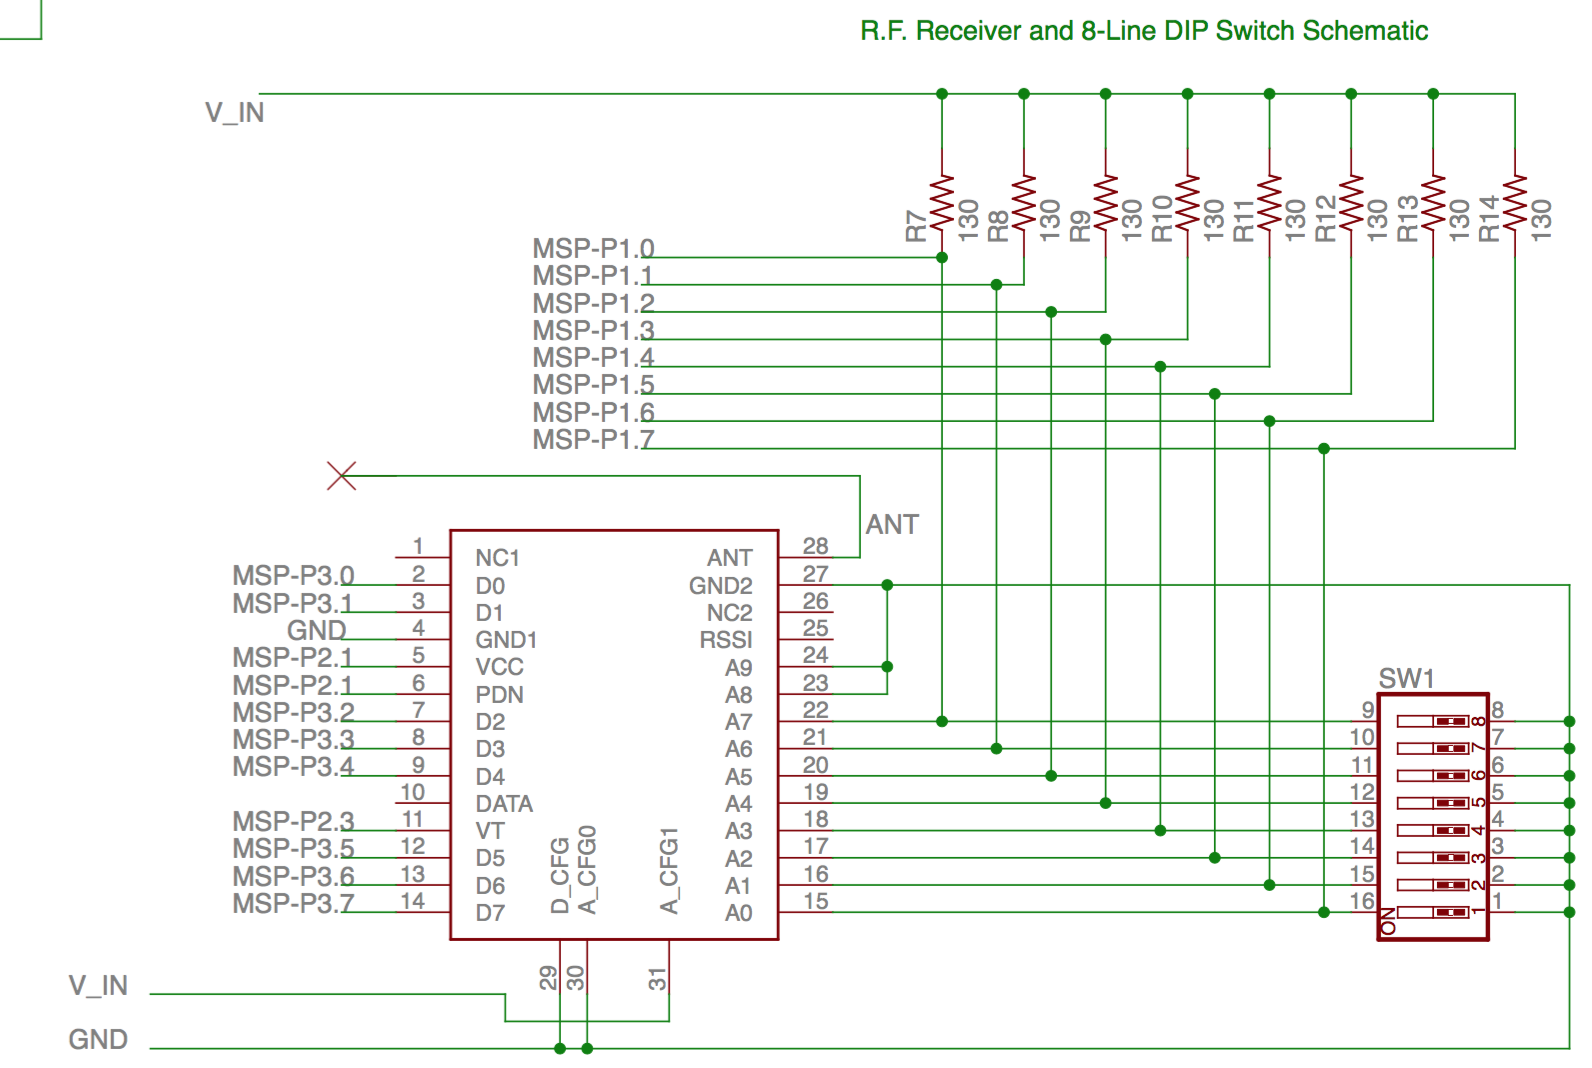
\includegraphics[scale=0.5]{receiver-dip-schematic.png}
	\caption{RF Receiver/Decoder and 8-Pin DIP Switch Schematic\label{fig:rf-receiver-decoder-schematic}}
\end{figure}

\begin{figure} [H]
	\centering
	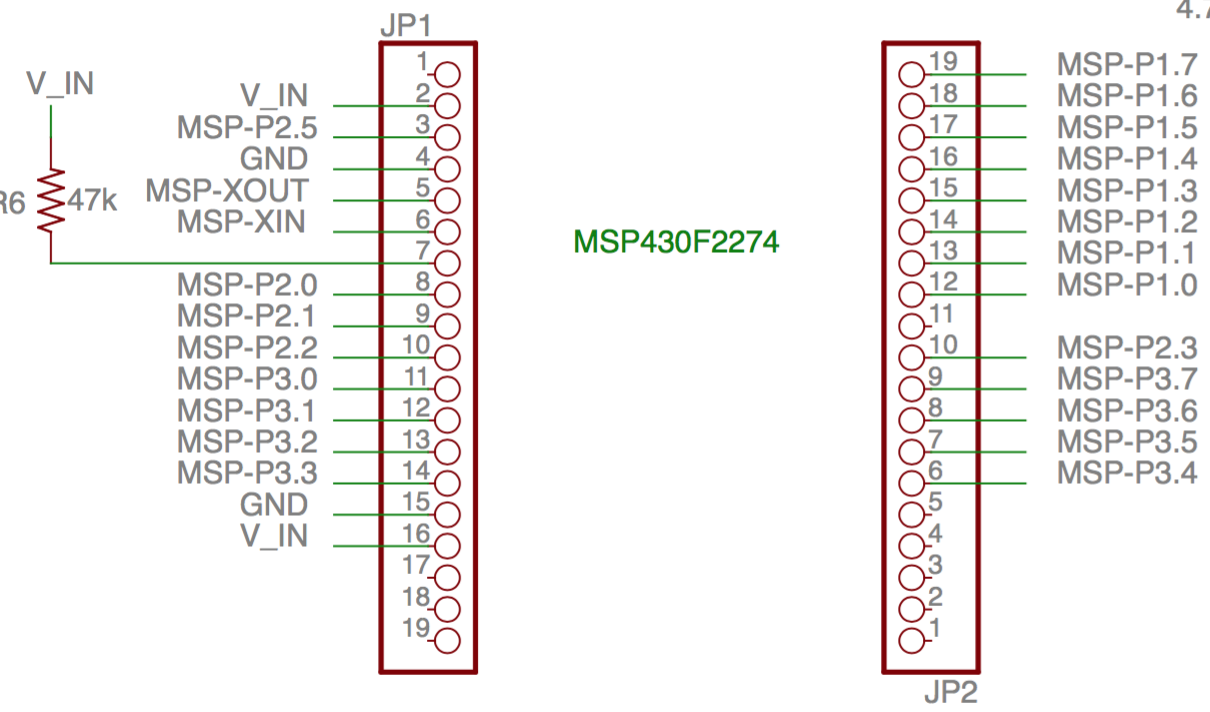
\includegraphics[scale=0.5]{msp-schematic.png}
	\caption{MSP430F2274 Schematic\label{fig:msp-schematic}}
\end{figure}


\subsubsection{System PCB Schematic}
Shown below in Figure \ref{fig:system-pcb} is the entire PCB schematic of the friendly interrogator unit. This is the initial revision and will only be utilized for testing and debugging the system. There are 3 sub-schematics that will be expanded upon below.
\begin{figure} [H]
	\centering
	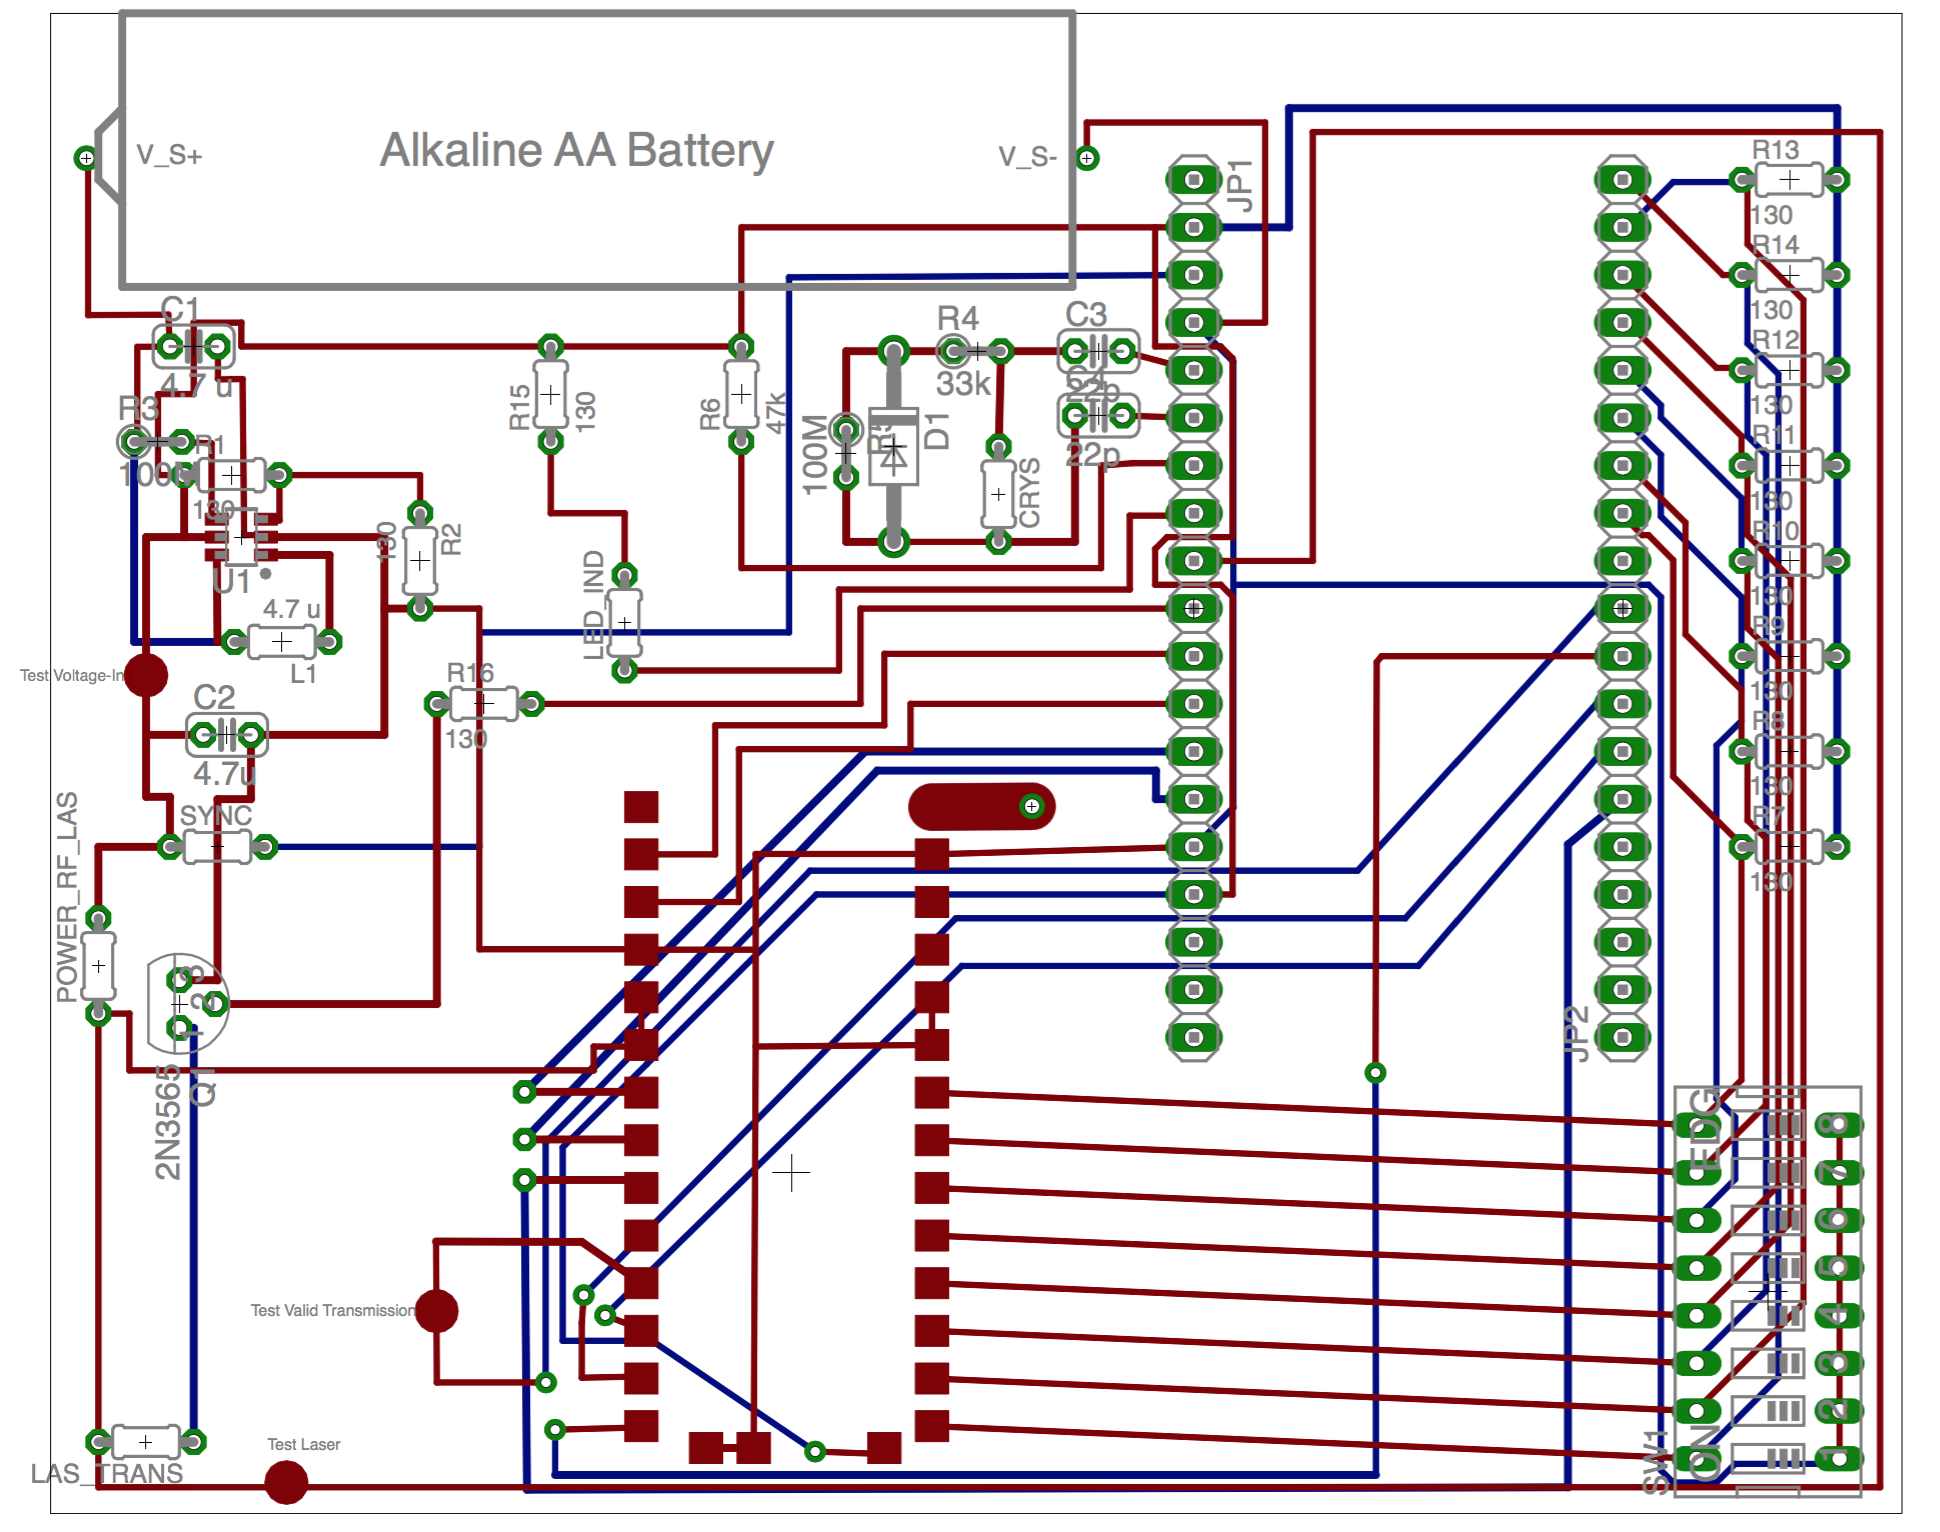
\includegraphics[scale=0.4]{system-pcb.png}
	\caption{Overall System PCB Schematic\label{fig:system-pcb}}
\end{figure}

\subsubsection{PCB Sub-Schematics and Verification}
This section is not intended to review every single component on the PCB, but rather is meant to highlight some of the schematics I will utilize throughout the testing of the friendly interrogator unit.

The MSP430F2274 will act as the main processing/control unit for all peripheral inputs and outputs. For this reason the PCB schematic for the MSP430 has been omitted and one may refer to the pin layout or the circuit schematic above in Figure \ref{fig:msp-schematic}. However, it should be noted that the MSP430 will not be soldered directly to the board, rather a "breakout" board will be utilized for programming/flashing the microcontroller (by using a breadboard with a FET Programmer). This is shown below in Figure \ref{fig:msp-breakout}.

\begin{figure} [H]
	\centering
	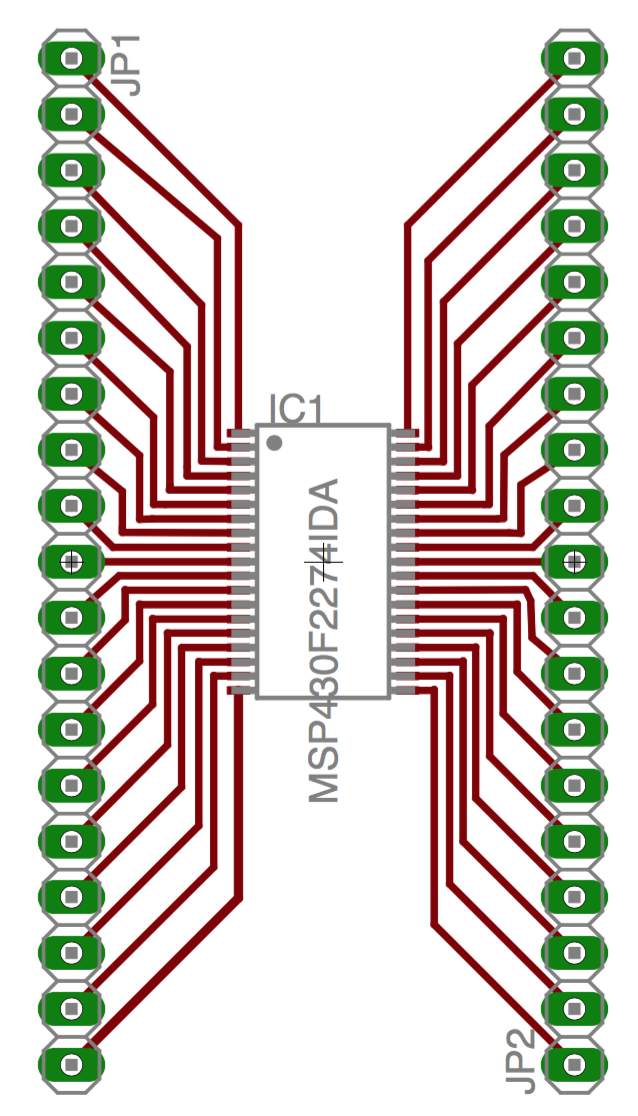
\includegraphics[scale=0.4]{msp-breakout.png}
	\caption{MSP430 TSSOP-to-DIP PCB Schematic\label{fig:msp-breakout}}
\end{figure}


 The voltage converter, the laser transmitter, and the R.F. receiver are the 3 sub-schematics that are of the utmost importance to the verification of the requirements. These are shown in Figure \ref{fig:converter-pcb}, \ref{fig:laser-pcb}, and \ref{fig:receiver-pcb} respectively. Above each schematic is an explanation of how the circuit will be used in the verification of the requirements for the friendly interrogator unit. 

\normalsize\textbf{Voltage Regulator}\\
The voltage regulator steps up the 1.5V AA battery source to 3.3V which is required to operate the MSP430, R.F. receiver, and the laser transmitter. The pad labeled as "Test Voltage-In" will be probed upon applying a 1.5V source to the top two vias on the PCB. This will ensure the voltage being supplied to the MSP430, R.F. receiver, and laser transmitter are all adequate and meet the requirements as stated. 

This verification will take place prior to soldering anything onto the board to ensure that no low/high voltages are being applied to the components when using them. The only component that will be on the board is the AAT1217 voltage regulator. Only upon verifying the output voltage ("Test Voltage-In") is 1.5V, will all other components be soldiered onto the board to continue testing. 
\begin{figure} [H]
	\centering
	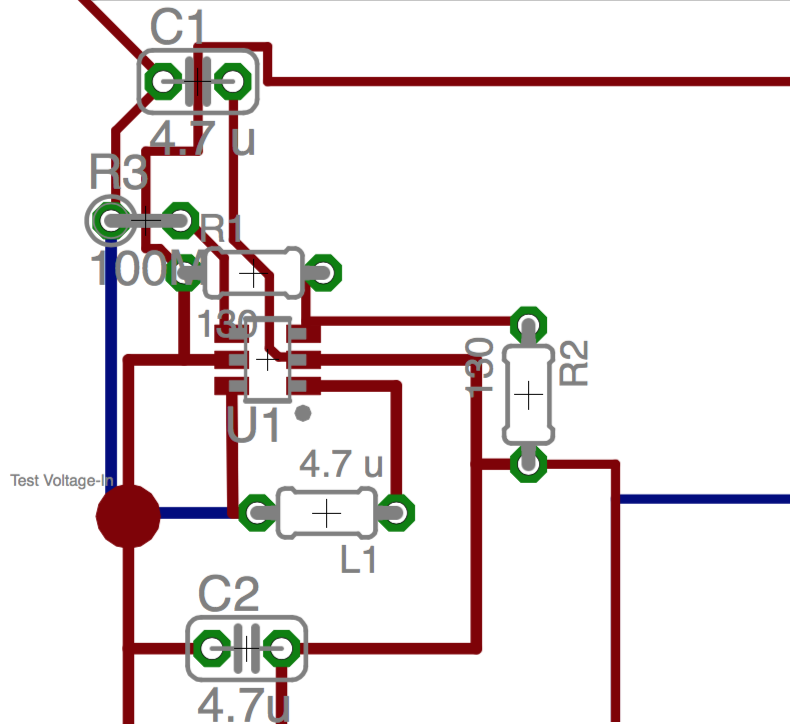
\includegraphics[scale=0.4]{converter-pcb.png}
	\caption{Voltage Converter PCB Schematic\label{fig:converter-pcb}}
\end{figure}

\normalsize\textbf{Laser Transmitter} \\
The laser transmitter will be necessary to pulse the unique I.D. of the interrogator to the friendly unit. This will be done at a 40kHz rate and generated by the MSP430. On the PCB, the pad labeled as "Test Laser" will be probed and connected to an oscilloscope to verify the rate of the signal being fed to the laser transmitter. 

This verification will take place prior to connecting the actual laser transmitter to the board in order to confirm that the desired rate of operation is 40kHz. This step will require the MSP430 to be flashed and programmed with the correct software to generate interrupts on the MSP-P2.1 line. Once it is verified that the "Test Laser" signal can be triggered "high" at a 40kHz rate, then the software can be written to implement the main I.F.F. features. ?????????????????
\begin{figure} [H]
	\centering
	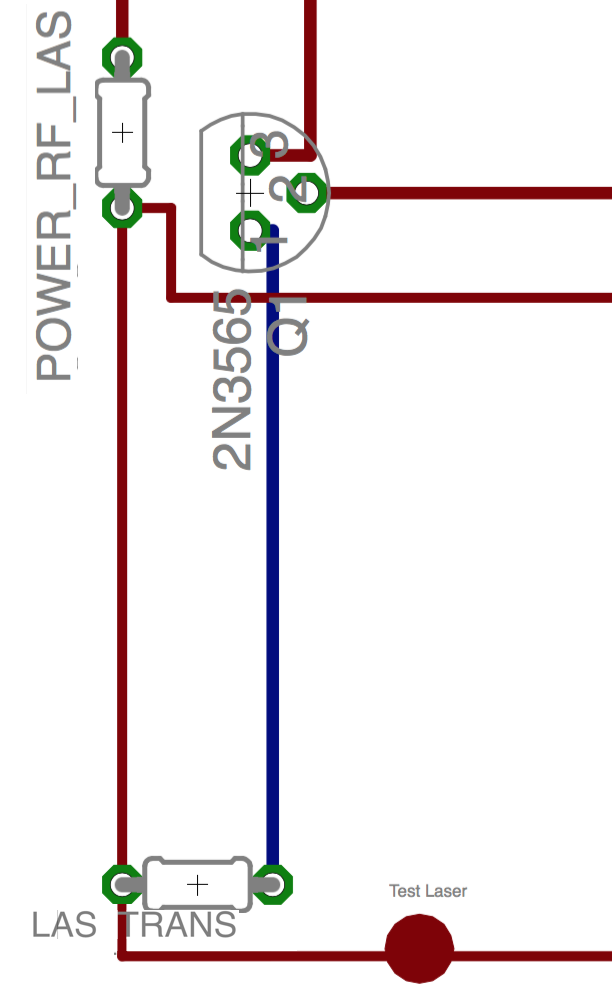
\includegraphics[scale=0.4]{transmitter-pcb.png}
	\caption{Laser Transmitter PCB Schematic\label{fig:laser-pcb}}
\end{figure}

\normalsize\textbf{R.F. Receiver} \\
Once the R.F. receiver gets a signal from the friendly target unit, it will set the "$V_{T}$ pin high. This will indicate to the MSP430 that new data is ready to be received from the KH3. Once the transmitter is set up properly by Noah, and the KH3 receiver has been properly tested on a breadboard, the receiver schematic can be tested (shown in Figure \ref{fig:receiver-pcb}). This will be done by sending a signal on the transmitter and verifying the "Test Valid Transmission" pad is high on the PCB. 

Another feature to note is the line running from the receiver to the connection for the antenna. This is a wider trace due to the impedence matching of 50 ohms. This is explained in the Design Review in the Calculations section. 
\begin{figure} [H]
	\centering
	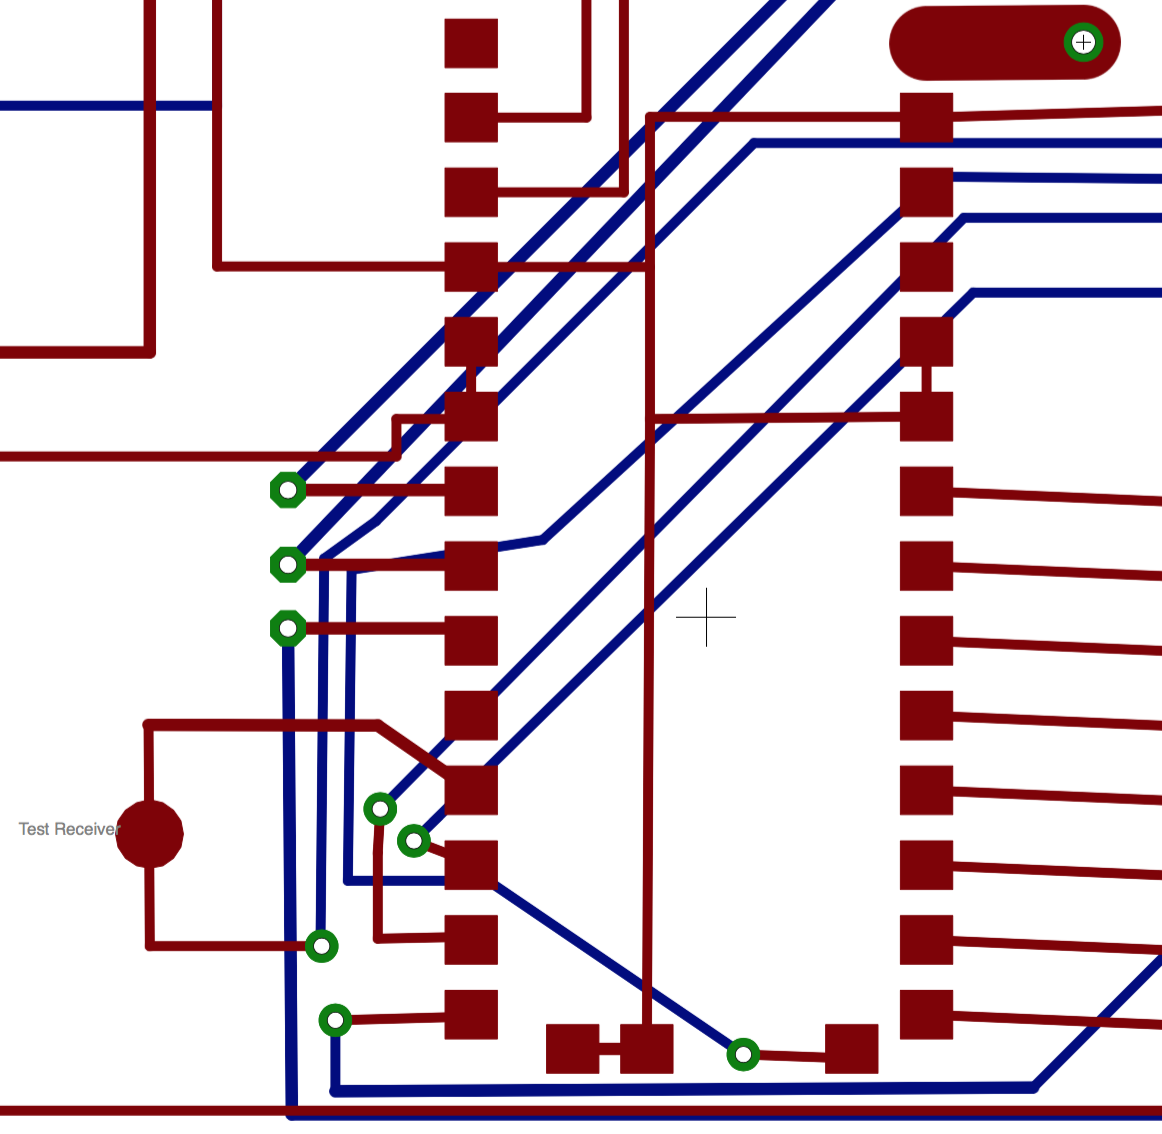
\includegraphics[scale=0.4]{receiver-antenna-pcb.png}
	\caption{R.F. Receiver/Antenna PCB Schematic\label{fig:receiver-pcb}}
\end{figure}


The KH3 transmitter first must be tested to verify that it is properly functioning before soldering to the friendly interrogator PCB. For this reason a breakout board to be used in conjunction with a breadboard was created to test. This is shown below in Figure \ref{fig:receiver-breakout}.

\begin{figure} [H]
	\centering
	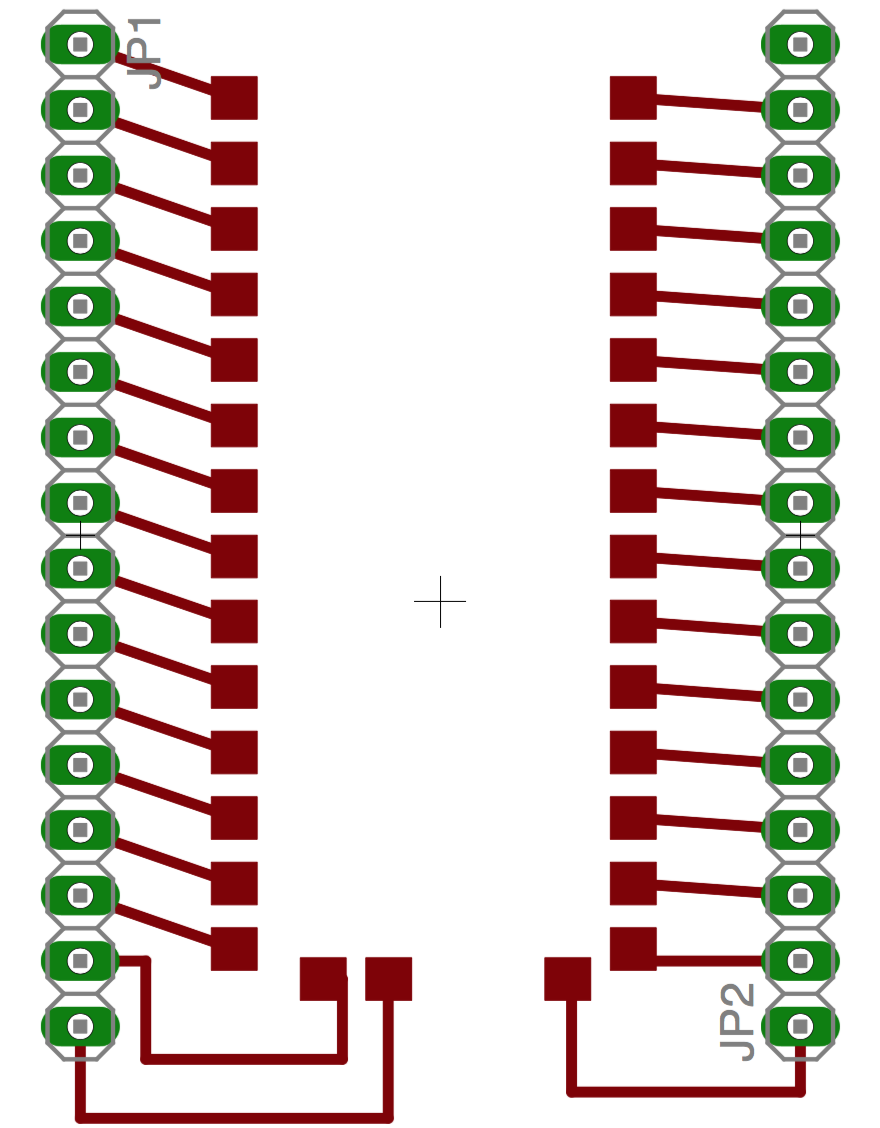
\includegraphics[scale=0.3]{kh3-receiver-breakout.png}
	\caption{R.F. Receiver/Antenna PCB Schematic\label{fig:receiver-breakout}}
\end{figure}


\subsubsection{Software} \label{section-software}
The software for the MSP430 is featured in the bottom Appendix section. Although this has not been debugged yet (for both its logic and syntax errors), the basic concept of flow is correct, and the comments explain what each line does. 


\subsection{Conclusion}
To summarize section 2.1.3 and 2.1.4, the necessary steps that must be taken over the next few weeks are as follows:

Upon receiving initial PCB:
\begin{enumerate}
	\item Solder AAT1217 Voltage Converter to proper connection on PCB.
	\item Apply 1.5V source voltage to V\_S+ and V\_S-.
	\item Verify 1.5V is being boosted to 3.3V by probing "Test Voltage-In" pad on PCB.
	\item Connect and solder MSP430F2274 to MSP Breakout Board (Figure \ref{fig:msp-breakout})
	\item Flash MSP430 with MSP FET Programming Tool/breadboard with appropriate software to generate interrupts at 40kHz rate on P2.1.
	\item Attach MSP430 to PCB and apply 1.5V to V\_S+ and V\_S-.
	\item Verify 40kHz rate by probing "Test Laser" with oscilloscope.
	\item Connect Linx KH3 to breakout board and begin testing with KH3 transmitter (partnered task - with Noah)
	\item Verify via the "Test Valid Transmission" line that a signal is properly being received from the transmitter. 
	\end{enumerate}

There have been some minor setbacks over the past couple weeks. This was partially due to a misconnection on one of our receivers that caused a signal to short, and the wrong part being ordered to connect from the MSP to a breadboard for testing. However the team has made this work up over the past week, ordered the correct parts and is still on pace to finish in time for final demonstration. There is still plenty of work to do in the next month, however, it is completely reasonable to finish this project in time (barring no major errors/setbacks).

I believe the work I have contributed relative to the project as a whole is completely fair and I believe it has been divided fairly equally. As shown above, I have spent a significant amount of time developing PCBs/Schematics in Eagle and I have also spent a significant amount of time developing the software for the friendly interrogator side. All together, I believe I have put in well over the estimated 13 hours/week Noah and I came up with at the beginning of the semester. I believe I have been putting in anywhere between 15-25 hours/week (fluctuating). 


%SECTION - References
\bibliographystyle{IEEE_ECE}
% include the BibTex file here to build reference
\bibliography{Citations}\addcontentsline{toc}{section}{Reference}
\clearpage
\section*{Appendix}
\begin{lstlisting}
//******************************************************************************
//  MSP430F2274 Infantry Identification Friend or Foe Software 
//  FRIENDLY INTERROGATOR UNIT
//  Author: Eric Meyers and Noah Prince
//  Date(s): Initial Revision 3/15/2016
// 
//  Description: This piece of software is an interrupt based piece of microcontroller... 
// INPUT GPIO PINS : P1.0, P1.1, P1.2, P1.3, P1.4, P1.5, P1.6, P1.7 = R.F. Address Lines
//                   P3.0, P3.1, P3.2, P3.3, P3.4, P3.5, P3.6, P3.7 = R.F. Data Lines
//                   P2.1 = Power Button for R.F. Receiver and Laser Transmitter
//                   P2.5 = Sync Button to Reset/Sync Clocks
//                   
//       
// OUTPUT GPIO PINS: P2.0 = LED Indicator (Friendly or Enemy)
//                   P2.2 = Laser Transmitter
//
//  Built with CCE Version: 3.2.2 and IAR Embedded Workbench Version: 4.11B
//******************************************************************************
#include <msp430.h>
#include "pins.h"

/* ==== Initialize Global Variables ==== */
int seconds = 0; //Seconds Timer 
int ten_seconds = 0; //Ten Second Timer

/*  Main Function
*  Description: This main function performs all necessary tasks to take in the 
*              appropriate address lines, pulse the appropriate unique I.D. to the
*              friendly target unit and wait for an acknowledgement. This "ack" from
*              the target unit
*/
int main(void)
{
/* ==== Initialize Local Variables ==== */
char address = 0;
char start = 0;
char check_sum = 0;
int i = 0;            //loop variable
int unique_id;

/* Turn off Watch-Dog Timers */
WDTCTL = WDTPW + WDTHOLD; 

/* ==== Set Direction of GPIO ==== */
//PXDIR - BITWISE : 1 OUTPUT 0 INPUT : source: page 329 MSP430x2xx  */
P1DIR |= 0xFFFF; // All pins on P1 (P1.0 - P1.7) are inputs - Address Lines
P3DIR |= 0xFFFF; // All pins on P3 (P3.0 - P3.7) are inputs - Data Lines
P2DIR &= (BIT0 | BIT2); //Set P2.0 & P2.2 as output - Laser Transmitter & Indicator
P2DIR |= (BIT1 | BIT5); //Set P2.1 & P2.5 as input - Sync and Power to R.F. & Laser

/* =======Laser Pulse Word ==========================================
---------------------------------------------------------------------
| ST_B3 | ST_B2 | ST_B1 | ST_B0 | A7 ... A0 | CS3 | CS2 | CS1 | CS0 |
---------------------------------------------------------------------
with ST_B3 - ST_B0 = Start Bits (Logic Highs (1s))
A7 - A0 = R.F. Address Lines (Depending on 8-Pin DIP Switch)
CS3 - CS0 = CheckSum Bits (Not Really sure what these are for yet tbh
======================================================================*/
//Combine address into single char to get a
address |= (P1IN & 0xFF);
start = 0x0F;

for(; i < 8; i++) {
check_sum += (address>>i) & BIT1;
}

//shift bits properly to set the unique_id upon starting
unique_id = (start << 12) | (address << 4) | check_sum;

/* ============ Setup Timers ===========================================*/
//Setup Timer A1 to perform 1 Hz interrupts (for seconds counter) - 1s
char ten_sec_timer_a_flag = 0;//Validation period flag - 10 seconds
TA0CCR0 = 32768; // Set count limit (32.768 kHz Clock = 32,768 ticks until one interrupt is registered)
TA0CCTL0 = 0x10; //Enable counter interrupts - bit 4
TA0CTL = TASSEL_1 + MC_1; //Timer A0 with ACLK @ 32768Hz @ 3.0V(VERIFY), count up.

//Setup Timer B0 to do 40 kHz interrupts (for laser) -  25us
char laser_timer_b_flag = 0;
TB0CCR0 = 100; // Set count limit (16 MHz Clock = 16000 ticks until one interrupt is registered)
TB0CCTL0 = 0x10; //Enable counter interrupts - bit 4
TB0CTL = TBSSEL_2 + ID_2 + MC_1; //Timer A0 with SMCLK @ 16 MHz/4 = 4MHz @ 3.0V(VERIFY), count up.


/* ==== Main Loop (Perform pulsing, poll for response?) ==== */
while (1)
{
/* FIRST: UPDATE ACKNOWLEDGEMENT PASSPHRASE */
if (ten_sec_timer_a_flag)
{
ten_sec_timer_a_flag = 0;
// UPDATE ACKNOWLEDGEMENT VERIFICATION PASSPHRASE
}

// Check to see if operator has switched R.F. and Laser ON
if (P2IN & BIT1) 
{
/* PULSE UNIQUE ID, CHECK VALID TRANSMISSION SIGNAL*/
for (i = 0; i < 16; i ++)
{
while (!laser_timer_b_flag);    //wait for 40kHz signal
laser_timer_b_flag = 0;         //reset flag

//Turn P2.2 ON or OFF depending on state of unique I.D.
((unique_id >> i) & BIT1) ? (P2OUT |= 0x02) : (P2OUT &= ~0x02);
}

/*CHECK R.F. RECEIVER VALID TRANSMISSION SIGNAL*/
if (P2IN & BIT3)
//WAIT FOR RESPONSE - TIMEOUT OF 40 ms?   
}
} 
}
// If V_IN_RF_LAS switch != high then enter LPM3 w/ interrupts enabled
//__bis_SR_register(LPM3_bits + GIE);
}  


/*  ISR : Timer_A3
*  Description: This timer acts as our "RTC" and increments the "seconds" variable every second,
*  (obviously), and also depending on the value of "seconds" it sets the ten_sec_timer_a_flag.
*/
#pragma vector = TIMER0_A0_VECTOR
__interrupt void Timer0_A0 (void) 
{
seconds++;
ten_sec_timer_a_flag = (seconds % 10 == 0);
}


/*  ISR : Timer_B3
*  Description: This timer triggers the laser transmitter at 40 kHz 
*/
#pragma vector = TIMER0_B0_VECTOR
__interrupt void Timer0_B0 (void) 
{
laser_timer_b_flag = 1; //Set the laser_timer_b_flag to 
}



\end{lstlisting}



\end{spacing}
\end{document}

